\documentclass{article}

\usepackage{graphicx}
\usepackage{tikz}
\usepackage{tikzsymbols}
\usetikzlibrary{calc,patterns,shapes.geometric}
\pagestyle{empty}
\usepackage[margin=0pt]{geometry}
\geometry{papersize={14in,12in}}

\def\centerarc[#1](#2)(#3:#4:#5){\draw[#1] ($(#2)+({#5*cos(#3)},{#5*sin(#3)})$) arc (#3:#4:#5);}

\begin{document}
	\begin{figure}
		\centering
		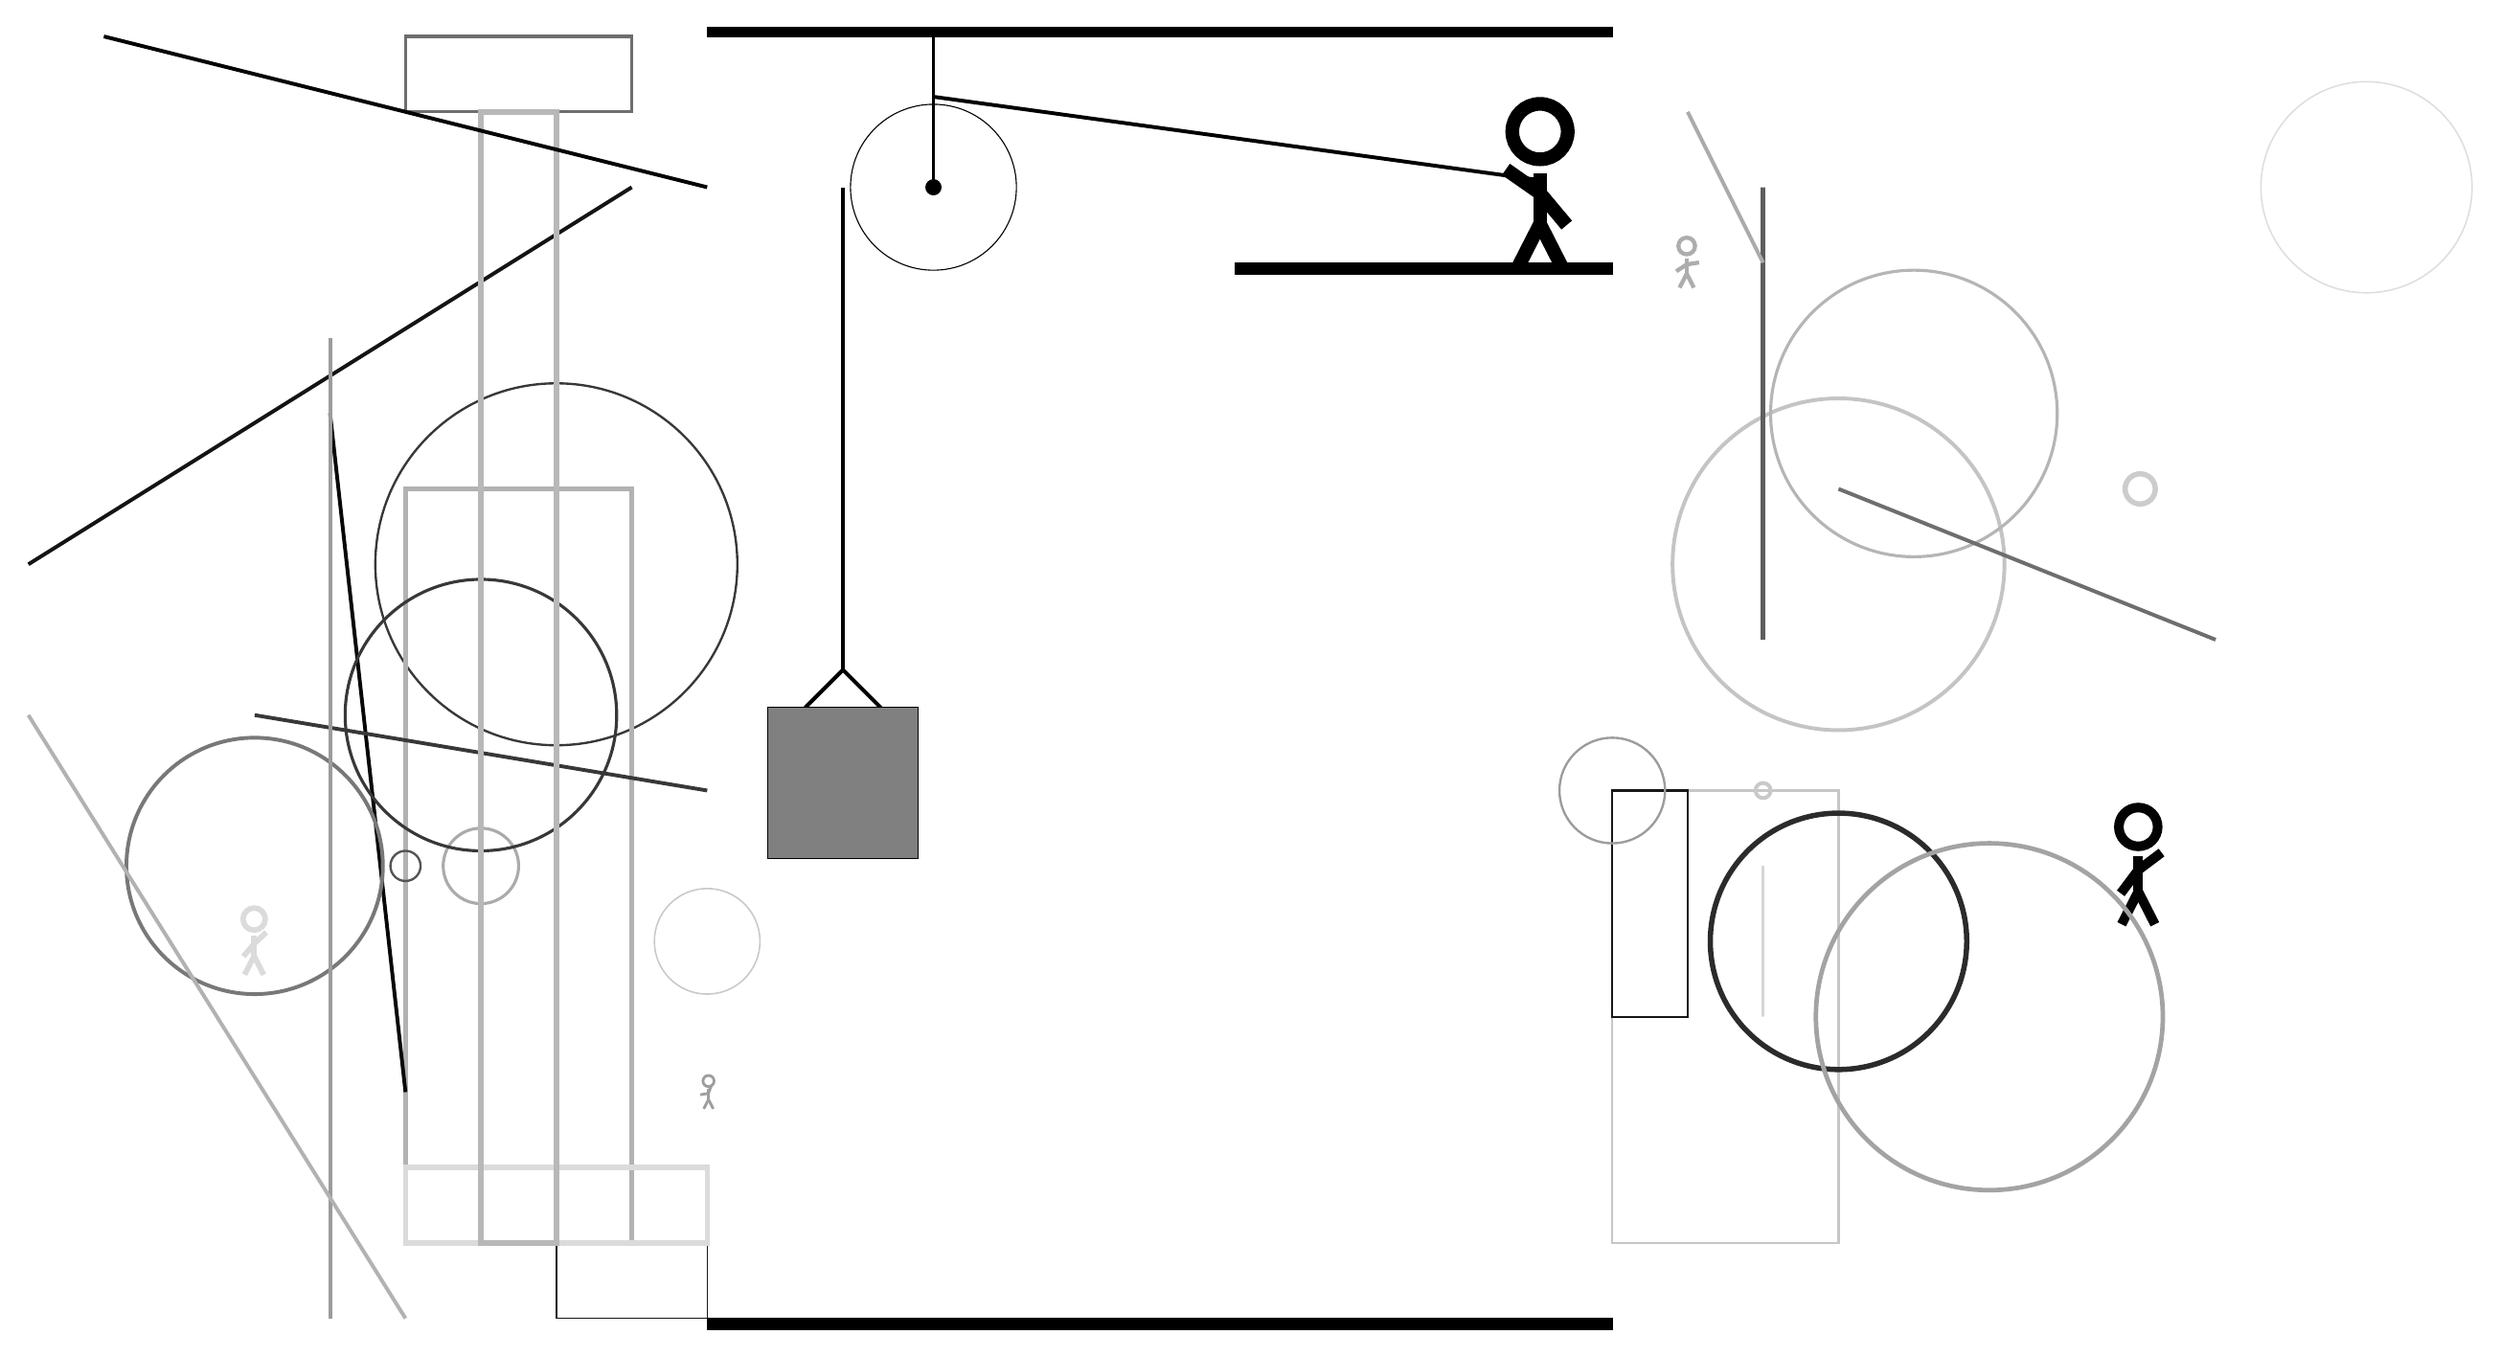
\begin{tikzpicture}
			%%%%% START %%%%%
			
			\draw[fill=black] (-2, 14) rectangle (10, 14.125);
			
			\draw (1, 12) circle (1.1);
			\draw[fill=black] (1, 12) circle (0.1);
			\draw[line width=0.5mm] (1, 14) -- (1, 12);
			
			\draw[line width=0.5mm](-0.7, 5.1) --  (-0.2, 5.6) -- (0.3, 5.1);
			\draw[fill=black!50] (-1.2, 5.1) rectangle (0.8, 3.1);
			
			\draw[line width=0.5mm](-0.2, 12) -- (-0.2, 5.6);
			\centerarc[line width=0.5mm](1, 12)(90:180:1.2000000000000002)
			\draw[line width=0.5mm](1, 13.2) -- (9, 12.1);
			
			\node at (9, 12) {\Strichmaxerl[10][-35][-50]};
			\draw[fill=black] (5, 11) rectangle (10, 10.85);
			
			\draw[line width=0.3mm, color=black!22] (10, 4) rectangle (13, -2);
			
			\draw [line width=0.3mm, color=black!78](-4, 7) circle (2.4);
			\draw[line width=0.6mm, color=black!30] (-3, -2) rectangle (-6, 8);
			\draw [line width=0.5mm, color=black!23](13, 7) circle (2.2);
			
			\draw[line width=0.3mm, color=black!91] (11, 4) rectangle (10, 1);
			\draw [line width=0.7mm, color=black!20](17, 8) circle (0.2);
			
			\draw [line width=0.7mm, color=black!83](13, 2) circle (1.7);
			\draw [line width=0.3mm, color=black!39](10, 4) circle (0.7);
			\draw [line width=0.4mm, color=black!33](-5, 3) circle (0.5);
			\draw [line width=0.2mm, color=black!13](20, 12) circle (1.4);
			\draw[line width=0.2mm, color=black!91] (-2, -3) rectangle (-4, -1);
			
			\draw [line width=0.4mm, color=black!29](14, 9) circle (1.9);
			\draw[line width=0.6mm, color=black!63] (12, 12) rectangle (12, 6);
			\draw[line width=0.5mm, color=black!97](-7, 9) -- (-6, 0);
			\draw [line width=0.4mm, color=black!78](-5, 5) circle (1.8);
			\node[line width=0.3mm, color=black!38] at (-2, 0) {\Strichmaxerl[2][10][70]};
			\draw[line width=0.3mm, color=black!16] (12, 1) rectangle (12, 3);
			\node[line width=0.5mm, color=black!32] at (11, 11) {\Strichmaxerl[3][33][9]};
			\draw[line width=0.5mm, color=black!78](-2, 4) -- (-8, 5);
			
			\draw [line width=0.5mm, color=black!53](-8, 3) circle (1.7);
			\draw[line width=0.7mm, color=black!14] (-2, -2) rectangle (-6, -1);
			
			\draw[line width=0.5mm, color=black!33](12, 11) -- (11, 13);
			\draw [line width=0.2mm, color=black!21](-2, 2) circle (0.7);
			\draw [line width=0.3mm, color=black!67](-6, 3) circle (0.2);
			\draw [line width=0.5mm, color=black!21](12, 4) circle (0.1);
			
			\draw[line width=0.5mm, color=black!92](-3, 12) -- (-11, 7);
			\node[line width=0.3mm, color=black!99] at (17, 3) {\Strichmaxerl[7][53][37]};
			\node[line width=0.3mm, color=black!14] at (-8, 2) {\Strichmaxerl[4][50][43]};
			
			\draw[line width=0.4mm, color=black!57] (-3, 14) rectangle (-6, 13);
			\draw[line width=0.5mm, color=black!57](13, 8) -- (18, 6);
			\draw[line width=0.7mm, color=black!28] (-4, 13) rectangle (-5, -2);
			
			\draw [line width=0.6mm, color=black!36](15, 1) circle (2.3);
			\draw[line width=0.5mm, color=black!39](-7, 10) -- (-7, -3);
			\draw[line width=0.5mm, color=black!99](-2, 12) -- (-10, 14);
			\draw[line width=0.5mm, color=black!30](-6, -3) -- (-11, 5);
			
			\draw[fill=black] (-2, -3) rectangle (10, -3.15);
			
			%%%%% END %%%%%
		\end{tikzpicture}
	\end{figure}	
\end{document}